% Options for packages loaded elsewhere
% Options for packages loaded elsewhere
\PassOptionsToPackage{unicode}{hyperref}
\PassOptionsToPackage{hyphens}{url}
\PassOptionsToPackage{dvipsnames,svgnames,x11names}{xcolor}
%
\documentclass[
  indonesian,
]{article}
\usepackage{xcolor}
\usepackage{amsmath,amssymb}
\setcounter{secnumdepth}{5}
\usepackage{iftex}
\ifPDFTeX
  \usepackage[T1]{fontenc}
  \usepackage[utf8]{inputenc}
  \usepackage{textcomp} % provide euro and other symbols
\else % if luatex or xetex
  \usepackage{unicode-math} % this also loads fontspec
  \defaultfontfeatures{Scale=MatchLowercase}
  \defaultfontfeatures[\rmfamily]{Ligatures=TeX,Scale=1}
\fi
\usepackage{lmodern}
\ifPDFTeX\else
  % xetex/luatex font selection
\fi
% Use upquote if available, for straight quotes in verbatim environments
\IfFileExists{upquote.sty}{\usepackage{upquote}}{}
\IfFileExists{microtype.sty}{% use microtype if available
  \usepackage[]{microtype}
  \UseMicrotypeSet[protrusion]{basicmath} % disable protrusion for tt fonts
}{}
\makeatletter
\@ifundefined{KOMAClassName}{% if non-KOMA class
  \IfFileExists{parskip.sty}{%
    \usepackage{parskip}
  }{% else
    \setlength{\parindent}{0pt}
    \setlength{\parskip}{6pt plus 2pt minus 1pt}}
}{% if KOMA class
  \KOMAoptions{parskip=half}}
\makeatother
% Make \paragraph and \subparagraph free-standing
\makeatletter
\ifx\paragraph\undefined\else
  \let\oldparagraph\paragraph
  \renewcommand{\paragraph}{
    \@ifstar
      \xxxParagraphStar
      \xxxParagraphNoStar
  }
  \newcommand{\xxxParagraphStar}[1]{\oldparagraph*{#1}\mbox{}}
  \newcommand{\xxxParagraphNoStar}[1]{\oldparagraph{#1}\mbox{}}
\fi
\ifx\subparagraph\undefined\else
  \let\oldsubparagraph\subparagraph
  \renewcommand{\subparagraph}{
    \@ifstar
      \xxxSubParagraphStar
      \xxxSubParagraphNoStar
  }
  \newcommand{\xxxSubParagraphStar}[1]{\oldsubparagraph*{#1}\mbox{}}
  \newcommand{\xxxSubParagraphNoStar}[1]{\oldsubparagraph{#1}\mbox{}}
\fi
\makeatother


\usepackage{longtable,booktabs,array}
\newcounter{none} % for unnumbered tables
\usepackage{calc} % for calculating minipage widths
% Correct order of tables after \paragraph or \subparagraph
\usepackage{etoolbox}
\makeatletter
\patchcmd\longtable{\par}{\if@noskipsec\mbox{}\fi\par}{}{}
\makeatother
% Allow footnotes in longtable head/foot
\IfFileExists{footnotehyper.sty}{\usepackage{footnotehyper}}{\usepackage{footnote}}
\makesavenoteenv{longtable}
\usepackage{graphicx}
\makeatletter
\newsavebox\pandoc@box
\newcommand*\pandocbounded[1]{% scales image to fit in text height/width
  \sbox\pandoc@box{#1}%
  \Gscale@div\@tempa{\textheight}{\dimexpr\ht\pandoc@box+\dp\pandoc@box\relax}%
  \Gscale@div\@tempb{\linewidth}{\wd\pandoc@box}%
  \ifdim\@tempb\p@<\@tempa\p@\let\@tempa\@tempb\fi% select the smaller of both
  \ifdim\@tempa\p@<\p@\scalebox{\@tempa}{\usebox\pandoc@box}%
  \else\usebox{\pandoc@box}%
  \fi%
}
% Set default figure placement to htbp
\def\fps@figure{htbp}
\makeatother


% definitions for citeproc citations
\NewDocumentCommand\citeproctext{}{}
\NewDocumentCommand\citeproc{mm}{%
  \begingroup\def\citeproctext{#2}\cite{#1}\endgroup}
\makeatletter
 % allow citations to break across lines
 \let\@cite@ofmt\@firstofone
 % avoid brackets around text for \cite:
 \def\@biblabel#1{}
 \def\@cite#1#2{{#1\if@tempswa , #2\fi}}
\makeatother
\newlength{\cslhangindent}
\setlength{\cslhangindent}{1.5em}
\newlength{\csllabelwidth}
\setlength{\csllabelwidth}{3em}
\newenvironment{CSLReferences}[2] % #1 hanging-indent, #2 entry-spacing
 {\begin{list}{}{%
  \setlength{\itemindent}{0pt}
  \setlength{\leftmargin}{0pt}
  \setlength{\parsep}{0pt}
  % turn on hanging indent if param 1 is 1
  \ifodd #1
   \setlength{\leftmargin}{\cslhangindent}
   \setlength{\itemindent}{-1\cslhangindent}
  \fi
  % set entry spacing
  \setlength{\itemsep}{#2\baselineskip}}}
 {\end{list}}
\usepackage{calc}
\newcommand{\CSLBlock}[1]{\hfill\break\parbox[t]{\linewidth}{\strut\ignorespaces#1\strut}}
\newcommand{\CSLLeftMargin}[1]{\parbox[t]{\csllabelwidth}{\strut#1\strut}}
\newcommand{\CSLRightInline}[1]{\parbox[t]{\linewidth - \csllabelwidth}{\strut#1\strut}}
\newcommand{\CSLIndent}[1]{\hspace{\cslhangindent}#1}

\ifLuaTeX
\usepackage[bidi=basic,shorthands=off,provide=*]{babel}
\else
\usepackage[bidi=default,shorthands=off,provide=*]{babel}
\fi
\ifLuaTeX
  \usepackage{selnolig} % disable illegal ligatures
\fi


\setlength{\emergencystretch}{3em} % prevent overfull lines

\providecommand{\tightlist}{%
  \setlength{\itemsep}{0pt}\setlength{\parskip}{0pt}}



 


\makeatletter
\@ifpackageloaded{caption}{}{\usepackage{caption}}
\AtBeginDocument{%
\ifdefined\contentsname
  \renewcommand*\contentsname{Daftar Isi}
\else
  \newcommand\contentsname{Daftar Isi}
\fi
\ifdefined\listfigurename
  \renewcommand*\listfigurename{Daftar Gambar}
\else
  \newcommand\listfigurename{Daftar Gambar}
\fi
\ifdefined\listtablename
  \renewcommand*\listtablename{Daftar Tabel}
\else
  \newcommand\listtablename{Daftar Tabel}
\fi
\ifdefined\figurename
  \renewcommand*\figurename{Gambar}
\else
  \newcommand\figurename{Gambar}
\fi
\ifdefined\tablename
  \renewcommand*\tablename{Tabel}
\else
  \newcommand\tablename{Tabel}
\fi
}
\@ifpackageloaded{float}{}{\usepackage{float}}
\floatstyle{ruled}
\@ifundefined{c@chapter}{\newfloat{codelisting}{h}{lop}}{\newfloat{codelisting}{h}{lop}[chapter]}
\floatname{codelisting}{Daftar}
\newcommand*\listoflistings{\listof{codelisting}{Daftar Daftar}}
\makeatother
\makeatletter
\makeatother
\makeatletter
\@ifpackageloaded{caption}{}{\usepackage{caption}}
\@ifpackageloaded{subcaption}{}{\usepackage{subcaption}}
\makeatother
\usepackage{bookmark}
\IfFileExists{xurl.sty}{\usepackage{xurl}}{} % add URL line breaks if available
\urlstyle{same}
% fallback for those not using the hyperref driver hyperxmp:
\makeatletter
\@ifundefined{xmpquote}{\newcommand{\xmpquote}[1]{#1}}{}
\makeatother
\hypersetup{
  pdftitle={Hubungan Skor Albumin-Bilirubin (ALBI) Pra-Terapi dengan Respon Radiologis Terapi Lenvatinib dalam Rentang 12--16 Minggu Pertama pada Karsinoma Sel Hati yang Tidak Dapat Direseksi},
  pdfauthor={Kadek Adit Wiryadana; Gde Somayana; I Komang Agus Wira Nugraha},
  pdflang={id},
  pdfkeywords={\xmpquote{karsinoma sel hati}, \xmpquote{skor
ALBI}, \xmpquote{lenvatinib}, \xmpquote{mRECIST}, \xmpquote{respon
radiologis}},
  colorlinks=true,
  linkcolor={blue},
  filecolor={Maroon},
  citecolor={Blue},
  urlcolor={Blue},
  pdfcreator={LaTeX via pandoc}}


\title{Hubungan Skor Albumin-Bilirubin (ALBI) Pra-Terapi dengan Respon
Radiologis Terapi Lenvatinib dalam Rentang 12--16 Minggu Pertama pada
Karsinoma Sel Hati yang Tidak Dapat Direseksi}
\author{Kadek Adit Wiryadana \and Gde Somayana \and I Komang Agus Wira
Nugraha}
\date{25 November 2026}
\begin{document}
\maketitle
\begin{abstract}
\textbf{Latar Belakang:} Karsinoma sel hati (KSH) sebagian besar
terdiagnosis pada stadium lanjut sehingga terapi sistemik lini pertama
seperti lenvatinib menjadi pilihan utama. Respon klinis terhadap
lenvatinib sangat bervariasi dan dipengaruhi cadangan fungsional hati.
Skor Albumin-Bilirubin (ALBI) menawarkan penilaian fungsi hati yang
objektif dibandingkan skor Child-Turcotte-Pugh (CTP).

\textbf{Metode:} Studi kohort retrospektif pada pasien KSH tidak dapat
direseksi (BCLC B non-kandidat kuratif/lokoregional dan BCLC C) yang
menerima terapi lenvatinib di RSUP Prof.~dr. I.G.N.G. Ngoerah periode 1
Januari 2023 hingga 31 Desember 2025. Penilaian luaran menggunakan
pendekatan \emph{intention-to-treat} (ITT) berdasarkan kriteria mRECIST
pada minggu ke-12 hingga ke-16 (Penyakit Terkontrol {[}CR/PR/SD{]} vs
Penyakit Progresif {[}PD/meninggal sebelum evaluasi CT{]}). Analisis
mencakup statistik deskriptif, bivariat (\emph{Chi-square}/\emph{Fisher
exact} dan \emph{Relative Risk}), penentuan titik potong variabel
numerik melalui kurva ROC/AUC, serta regresi logistik biner multivariat.

\textbf{Hasil:} {[}Terisi otomatis setelah hasil render diverifikasi{]}

\textbf{Simpulan:} {[}Terisi otomatis setelah hasil akhir
diverifikasi{]}
\end{abstract}


\section{Audit Kelengkapan Data \& Validasi
Formula}\label{audit-kelengkapan-data-validasi-formula}

\begin{longtable}[]{@{}lrrl@{}}

\caption{\label{tbl-audit-data}Audit Kelengkapan Data (Missingness) dan
Verifikasi Kalkulasi pada Sampel Teranalisis.}

\tabularnewline

\toprule\noalign{}
Variabel & Terisi\_n & Missing\_n & Missing\_Pct \\
\midrule\noalign{}
\endhead
\bottomrule\noalign{}
\endlastfoot
Usia\_Num & 75 & 0 & 0.0\% \\
Jenis\_Kelamin & 75 & 0 & 0.0\% \\
BCLC\_Kat & 70 & 5 & 6.7\% \\
Etiologi\_Kat & 75 & 0 & 0.0\% \\
CTP\_Kat & 75 & 0 & 0.0\% \\
ECOG\_Kat & 75 & 0 & 0.0\% \\
Albumin\_gdL & 75 & 0 & 0.0\% \\
Bilirubin\_mgdL & 75 & 0 & 0.0\% \\
Skor\_ALBI & 75 & 0 & 0.0\% \\
AFP\_ng\_Num & 75 & 0 & 0.0\% \\
PIVKA\_Num & 5 & 70 & 93.3\% \\
Skor\_PNI & 75 & 0 & 0.0\% \\
UpToSeven\_Kat & 75 & 0 & 0.0\% \\
mCCI\_Num & 75 & 0 & 0.0\% \\
RDI\_12m & 74 & 1 & 1.3\% \\
Respon\_Kat & 75 & 0 & 0.0\% \\

\end{longtable}

Status Keputusan Riwayat Terapi Sebelumnya: Jumlah sampel tanpa riwayat
terapi sebelumnya (n = 75) memenuhi target minimal (n \textgreater= 68),
sehingga 4 pasien dengan riwayat TACE/reseksi/ablasi dieksklusi.

Validasi Formula (R vs Sheet): Jumlah baris dengan selisih bermakna pada
Skor ALBI (\(>0{,}05\)) = 1, PNI (\(>0{,}2\)) = 1, dan RDI (\(>1\%\)) =
0.

Validasi Skor mCCI: Rentang terukur 5-- 10 (jumlah pasien dengan skor
\(> 5\) = 64).

\begin{longtable}[]{@{}
  >{\raggedright\arraybackslash}p{(\linewidth - 6\tabcolsep) * \real{0.2632}}
  >{\raggedright\arraybackslash}p{(\linewidth - 6\tabcolsep) * \real{0.4342}}
  >{\raggedright\arraybackslash}p{(\linewidth - 6\tabcolsep) * \real{0.2632}}
  >{\raggedleft\arraybackslash}p{(\linewidth - 6\tabcolsep) * \real{0.0395}}@{}}

\caption{\label{tbl-audit-mrecist}Pemetaan Nilai Mentah MRECIST\_HASIL
ke Kategori Luaran ITT.}

\tabularnewline

\toprule\noalign{}
\begin{minipage}[b]{\linewidth}\raggedright
MRECIST\_Raw
\end{minipage} & \begin{minipage}[b]{\linewidth}\raggedright
Respon\_Detail
\end{minipage} & \begin{minipage}[b]{\linewidth}\raggedright
Respon\_Kat
\end{minipage} & \begin{minipage}[b]{\linewidth}\raggedleft
n
\end{minipage} \\
\midrule\noalign{}
\endhead
\bottomrule\noalign{}
\endlastfoot
Progressive Disease & PD (CT Evaluasi) & Penyakit Progresif & 30 \\
(Kosong) & Meninggal / Tanpa CT (ITT -\textgreater{} PD) & Penyakit
Progresif & 18 \\
Stable Disease & SD & Penyakit Terkontrol & 18 \\
Partial Response & PR & Penyakit Terkontrol & 7 \\
Complete Response & CR & Penyakit Terkontrol & 2 \\

\end{longtable}

\section{Pendahuluan}\label{pendahuluan}

Karsinoma sel hati (KSH) merupakan keganasan hati primer paling dominan
(85\%--90\% kasus) yang sebagian besar terdiagnosis pada stadium
menengah hingga lanjut sehingga membutuhkan terapi sistemik lini pertama
seperti lenvatinib (Kudo dkk., 2018; Perhimpunan Peneliti Hati
Indonesia, 2017). Cadangan fungsional hati residual berperan krusial
dalam menentukan tolerabilitas dosis dan respon antitumor. Skor
Albumin-Bilirubin (ALBI) menawarkan penilaian objektif berbasis albumin
serum dan bilirubin total tanpa bias subjektif skor Child-Turcotte-Pugh
(CTP) (Johnson dkk., 2015). Penelitian ini bertujuan menganalisis
hubungan skor ALBI pra-terapi dengan respon radiologis mRECIST dalam
rentang 12--16 minggu pertama terapi lenvatinib pada pasien KSH tidak
dapat direseksi di RSUP Prof.~dr. I.G.N.G. Ngoerah Denpasar.

\section{Metode}\label{metode}

Penelitian ini merupakan studi analitik kohort retrospektif berbasis
rekam medis pada pasien KSH tidak dapat direseksi (BCLC B non-kandidat
terapi kuratif/lokoregional dan BCLC C) usia \(\ge 18\) tahun yang
memulai terapi lenvatinib di RSUP Prof.~dr. I.G.N.G. Ngoerah Denpasar
periode 1 Januari 2023 hingga 31 Desember 2025 dengan target besar
sampel minimal 68 pasien. Kriteria eksklusi mencakup riwayat
transplantasi hati, kehamilan selama perawatan, serta penghentian terapi
\(< 12\) minggu di luar kejadian kematian. Evaluasi luaran mengikuti
prinsip intention-to-treat (ITT), yakni pasien yang meninggal sebelum
menjalani CT evaluasi minggu ke-12--16 diklasifikasikan sebagai penyakit
progresif. Dosis standar penyebut Relative Dose Intensity (RDI) 12
minggu ditetapkan berdasarkan berat badan
(\(\ge 60\text{ kg}: 12\text{ mg/hari}\);
\(< 60\text{ kg}: 8\text{ mg/hari}\)). Seluruh pengolahan data dilakukan
menggunakan RStudio dan Quarto dengan uji normalitas Shapiro--Wilk,
kurva ROC/AUC untuk penentuan cut-off variabel numerik, uji
Chi-square/Fisher exact beserta Relative Risk (RR), serta regresi
logistik biner multivariat beserta uji Variance Inflation Factor (VIF)
untuk mendeteksi multikolinearitas antar skor fungsi hati/nutrisi (ALBI,
CTP, dan PNI).

\section{Hasil}\label{hasil}

\subsection{Alur Seleksi Sampel dan Karakteristik
Subjek}\label{alur-seleksi-sampel-dan-karakteristik-subjek}

Dari total r n\_terjangkau data pasien pada tab MAIN\_60, didapatkan 75
subjek yang memenuhi kriteria analisis akhir (Jumlah sampel tanpa
riwayat terapi sebelumnya (n = 75) memenuhi target minimal (n
\textgreater= 68), sehingga 4 pasien dengan riwayat TACE/reseksi/ablasi
dieksklusi.), terdiri atas 18 pasien pada kelompok ALBI Derajat 1 dan 57
pasien pada kelompok ALBI Derajat 2--3 (Gambar~\ref{fig-alur}). Sebanyak
18 pasien tidak menjalani evaluasi CT 12--16 minggu
(meninggal/perburukan klinis) dan dikategorikan sebagai penyakit
progresif sesuai pendekatan ITT. Karakteristik dasar subjek disajikan
pada Tabel~\ref{tbl-karakteristik}.

\begin{figure}

\centering{

\pandocbounded{\includegraphics[keepaspectratio]{index_files/figure-pdf/fig-alur-1.pdf}}

}

\caption{\label{fig-alur}Diagram alur seleksi sampel penelitian
berdasarkan skor ALBI pra-terapi dan luaran respon radiologis mRECIST
12--16 minggu (ITT).}

\end{figure}%

\begin{longtable}[]{@{}
  >{\raggedright\arraybackslash}p{(\linewidth - 4\tabcolsep) * \real{0.4375}}
  >{\raggedright\arraybackslash}p{(\linewidth - 4\tabcolsep) * \real{0.1000}}
  >{\raggedright\arraybackslash}p{(\linewidth - 4\tabcolsep) * \real{0.4625}}@{}}

\caption{\label{tbl-karakteristik}Karakteristik Demografi, Klinis,
Laboratorium, dan Respon Terapi Subjek Penelitian.}

\tabularnewline

\toprule\noalign{}
\begin{minipage}[b]{\linewidth}\raggedright
Karakteristik
\end{minipage} & \begin{minipage}[b]{\linewidth}\raggedright
n Valid
\end{minipage} & \begin{minipage}[b]{\linewidth}\raggedright
Nilai / n (\%)
\end{minipage} \\
\midrule\noalign{}
\endhead
\bottomrule\noalign{}
\endlastfoot
Usia saat diagnosis (tahun) & 75 & 55.53 ± 11.35 (Rerata ± SD) \\
\textbf{Jenis Kelamin} & 75 & \\
--- Perempuan & & 17 (22.7\%) \\
--- Laki-laki & & 58 (77.3\%) \\
\textbf{Stadium BCLC} & 70 & \\
--- BCLC C & & 53 (75.7\%) \\
--- BCLC B & & 17 (24.3\%) \\
\textbf{Etiologi KSH} & 75 & \\
--- Non-viral & & 25 (33.3\%) \\
--- Viral & & 50 (66.7\%) \\
\textbf{Skor Child-Pugh (CTP)} & 75 & \\
--- CTP B-C & & 29 (38.7\%) \\
--- CTP A & & 46 (61.3\%) \\
\textbf{Status Performa ECOG} & 75 & \\
--- ECOG \textgreater= 2 & & 11 (14.7\%) \\
--- ECOG 0-1 & & 64 (85.3\%) \\
Albumin serum (g/dL) & 75 & 3.60 (2.90--4.00) (Median {[}IQR{]}) \\
Bilirubin total (mg/dL) & 75 & 1.20 (0.70--1.66) (Median {[}IQR{]}) \\
Skor ALBI pra-terapi & 75 & -2.22 (-2.51---1.66) (Median {[}IQR{]}) \\
\textbf{Derajat ALBI (1 / 2 / 3)} & 75 & \\
--- Derajat 1 & & 18 (24.0\%) \\
--- Derajat 2 & & 41 (54.7\%) \\
--- Derajat 3 & & 16 (21.3\%) \\
\textbf{Kategori Skor ALBI (Utama)} & 75 & \\
--- ALBI Derajat 2-3 & & 57 (76.0\%) \\
--- ALBI Derajat 1 & & 18 (24.0\%) \\
Kadar AFP pra-terapi (ng/mL) & 75 & 107.93 (6.61--2000.00) (Median
{[}IQR{]}) \\
\textbf{Kategori AFP} & 75 & \\
--- AFP \textgreater=200 ng/mL & & 36 (48.0\%) \\
--- AFP \textless200 ng/mL & & 39 (52.0\%) \\
Kadar PIVKA-II pra-terapi (mAU/mL) & 5 & 28.00 (10.00--42.25) (Median
{[}IQR{]}) \\
\textbf{Kategori PIVKA-II} & 5 & \\
--- PIVKA-II \textgreater=40 mAU/mL & & 2 (40.0\%) \\
--- PIVKA-II \textless40 mAU/mL & & 3 (60.0\%) \\
Prognostic Nutritional Index (PNI) & 75 & 42.63 ± 9.99 (Rerata ± SD) \\
\textbf{Kategori PNI} & 75 & \\
--- PNI Buruk (\textless49.75) & & 56 (74.7\%) \\
--- PNI Baik (\textgreater=49.75) & & 19 (25.3\%) \\
\textbf{Kriteria Up-to-Seven} & 75 & \\
--- Tidak Sesuai (\textgreater7) & & 65 (86.7\%) \\
--- Sesuai (\textless=7) & & 10 (13.3\%) \\
Skor mCCI & 75 & 6.00 (6.00--8.00) (Median {[}IQR{]}) \\
\textbf{Kategori Komorbiditas (mCCI)} & 75 & \\
--- mCCI Tinggi (\textgreater=2) & & 75 (100.0\%) \\
--- mCCI Rendah (0-1) & & 0 ( 0.0\%) \\
RDI 12 minggu (\%) & 74 & 100.00 (71.43--100.00) (Median {[}IQR{]}) \\
\textbf{Kategori RDI 12 minggu} & 74 & \\
--- RDI \textless=66.7\% & & 15 (20.3\%) \\
--- RDI \textgreater66.7\% & & 59 (79.7\%) \\
\textbf{Riwayat Terapi Sebelumnya} & 75 & \\
--- Ada Riwayat TACE/Reseksi/Ablasi & & 0 ( 0.0\%) \\
--- Naif Terapi & & 75 (100.0\%) \\
\textbf{Status Evaluasi 12--16 Minggu} & 75 & \\
--- CT Evaluasi 12-16 Minggu & & 57 (76.0\%) \\
--- Tanpa CT / Meninggal (ITT -\textgreater{} PD) & & 18 (24.0\%) \\
\textbf{Detail Respon mRECIST} & 75 & \\
--- CR & & 2 ( 2.7\%) \\
--- Meninggal / Tanpa CT (ITT -\textgreater{} PD) & & 18 (24.0\%) \\
--- PD (CT Evaluasi) & & 30 (40.0\%) \\
--- PR & & 7 ( 9.3\%) \\
--- SD & & 18 (24.0\%) \\
\textbf{Luaran Respon Terapi (Utama)} & 75 & \\
--- Penyakit Progresif & & 48 (64.0\%) \\
--- Penyakit Terkontrol & & 27 (36.0\%) \\

\end{longtable}

\subsection{Penentuan Titik Potong Variabel Numerik (Kurva
ROC/AUC)}\label{penentuan-titik-potong-variabel-numerik-kurva-rocauc}

Kurva ROC variabel usia menghasilkan AUC sebesar 0.568 (95\% CI:
0.432--0.704) dengan titik potong optimal 43 tahun (sensitivitas 22.2\%,
spesifisitas 91.7\%). Skor ALBI kontinu menunjukkan AUC sebesar 0.525
(95\% CI: 0.381--0.669) dengan titik potong empiris -2.80
(Gambar~\ref{fig-roc}).

\begin{figure}

\centering{

\pandocbounded{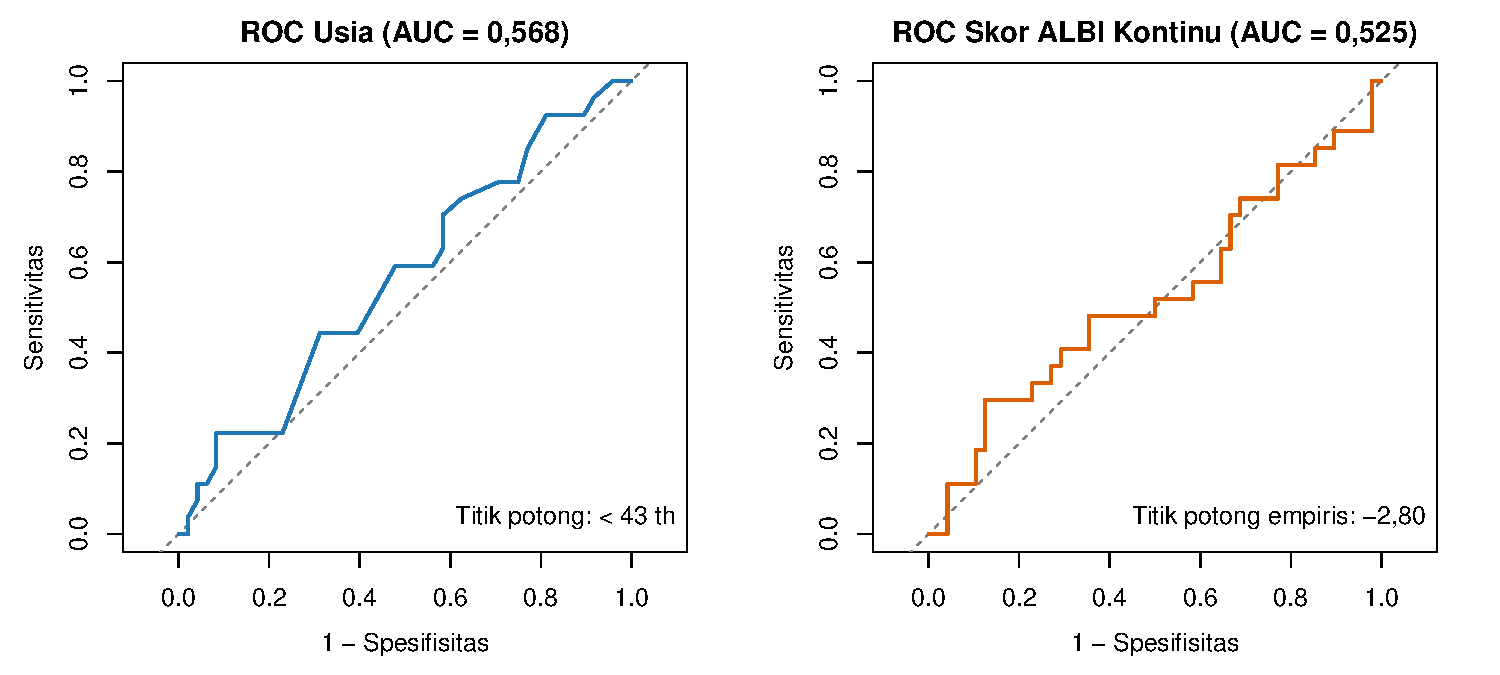
\includegraphics[keepaspectratio]{index_files/figure-pdf/fig-roc-1.pdf}}

}

\caption{\label{fig-roc}Kurva ROC penentuan titik potong usia (kiri) dan
evaluasi diskriminasi skor ALBI kontinu (kanan) dalam memprediksi
penyakit terkontrol.}

\end{figure}%

\subsection{Analisis Bivariat}\label{analisis-bivariat}

Secara keseluruhan, penyakit terkontrol tercapai pada 36.0\% (27/75
pasien). Pada kelompok ALBI Derajat 1, penyakit terkontrol tercapai pada
8/18 (44.4\%), dibandingkan 19/57 (33.3\%) pada ALBI Derajat 2--3,
dengan Relative Risk (RR) sebesar 1.33 (95\% CI: 0.71--2.51; \(p =\)
0.392) (Tabel~\ref{tbl-bivariat}; Gambar~\ref{fig-proporsi-albi}).

\begin{longtable}[]{@{}
  >{\raggedright\arraybackslash}p{(\linewidth - 14\tabcolsep) * \real{0.2299}}
  >{\raggedleft\arraybackslash}p{(\linewidth - 14\tabcolsep) * \real{0.0172}}
  >{\raggedright\arraybackslash}p{(\linewidth - 14\tabcolsep) * \real{0.2529}}
  >{\raggedright\arraybackslash}p{(\linewidth - 14\tabcolsep) * \real{0.1494}}
  >{\raggedright\arraybackslash}p{(\linewidth - 14\tabcolsep) * \real{0.1322}}
  >{\raggedright\arraybackslash}p{(\linewidth - 14\tabcolsep) * \real{0.0977}}
  >{\raggedright\arraybackslash}p{(\linewidth - 14\tabcolsep) * \real{0.0460}}
  >{\raggedright\arraybackslash}p{(\linewidth - 14\tabcolsep) * \real{0.0747}}@{}}

\caption{\label{tbl-bivariat}Hasil Analisis Bivariat Hubungan Skor ALBI
dan Variabel Perancu terhadap Penyakit Terkontrol (mRECIST 12--16
Minggu).}

\tabularnewline

\toprule\noalign{}
\begin{minipage}[b]{\linewidth}\raggedright
Variabel
\end{minipage} & \begin{minipage}[b]{\linewidth}\raggedleft
n
\end{minipage} & \begin{minipage}[b]{\linewidth}\raggedright
Perbandingan Kategori
\end{minipage} & \begin{minipage}[b]{\linewidth}\raggedright
Terkontrol (Kelompok Uji)
\end{minipage} & \begin{minipage}[b]{\linewidth}\raggedright
Terkontrol (Referensi)
\end{minipage} & \begin{minipage}[b]{\linewidth}\raggedright
RR (95\% CI)
\end{minipage} & \begin{minipage}[b]{\linewidth}\raggedright
Nilai p
\end{minipage} & \begin{minipage}[b]{\linewidth}\raggedright
Metode Uji
\end{minipage} \\
\midrule\noalign{}
\endhead
\bottomrule\noalign{}
\endlastfoot
Skor ALBI Pra-Terapi & 75 & ALBI Derajat 1 vs ALBI Derajat 2-3 & 8/18
(44.4\%) & 19/57 (33.3\%) & 1.33 (0.71--2.51) & 0.392 & Chi-square \\
Usia (cut-off ROC 43 th) & 75 & \textless{} 43 tahun vs \textgreater= 43
tahun & 6/10 (60.0\%) & 21/65 (32.3\%) & 1.86 (1.00--3.44) & 0.154 &
Fisher Exact \\
Jenis Kelamin & 75 & Laki-laki vs Perempuan & 20/58 (34.5\%) & 7/17
(41.2\%) & 0.84 (0.43--1.64) & 0.613 & Chi-square \\
Stadium BCLC & 70 & BCLC B vs BCLC C & 4/17 (23.5\%) & 18/53 (34.0\%) &
0.69 (0.27--1.77) & 0.420 & Chi-square \\
Etiologi KSH & 75 & Viral vs Non-viral & 17/50 (34.0\%) & 10/25 (40.0\%)
& 0.85 (0.46--1.57) & 0.610 & Chi-square \\
Skor Child-Pugh (CTP) & 75 & CTP A vs CTP B-C & 19/46 (41.3\%) & 8/29
(27.6\%) & 1.50 (0.76--2.96) & 0.228 & Chi-square \\
Status Performa ECOG & 75 & ECOG 0-1 vs ECOG \textgreater= 2 & 22/64
(34.4\%) & 5/11 (45.5\%) & 0.76 (0.36--1.57) & 0.511 & Fisher Exact \\
Kadar AFP Pra-Terapi & 75 & AFP \textless200 ng/mL vs AFP
\textgreater=200 ng/mL & 18/39 (46.2\%) & 9/36 (25.0\%) & 1.85
(0.95--3.57) & 0.057 & Chi-square \\
Kadar PIVKA-II Pra-Terapi & 5 & PIVKA-II \textless40 mAU/mL vs PIVKA-II
\textgreater=40 mAU/mL & 1/3 (33.3\%) & 2/2 (100.0\%) & 0.45
(0.12--1.76) & 0.400 & Fisher Exact \\
Prognostic Nutritional Index (PNI) & 75 & PNI Baik (\textgreater=49.75)
vs PNI Buruk (\textless49.75) & 9/19 (47.4\%) & 18/56 (32.1\%) & 1.47
(0.80--2.71) & 0.232 & Chi-square \\
Beban Tumor (Up-to-Seven) & 75 & Sesuai (\textless=7) vs Tidak Sesuai
(\textgreater7) & 7/10 (70.0\%) & 20/65 (30.8\%) & 2.28 (1.32--3.93) &
0.030 & Fisher Exact \\
Relative Dose Intensity (RDI 12 Minggu) & 74 & RDI \textgreater66.7\% vs
RDI \textless=66.7\% & 22/59 (37.3\%) & 5/15 (33.3\%) & 1.12
(0.51--2.46) & 0.776 & Chi-square \\

\end{longtable}

\begin{figure}

\centering{

\pandocbounded{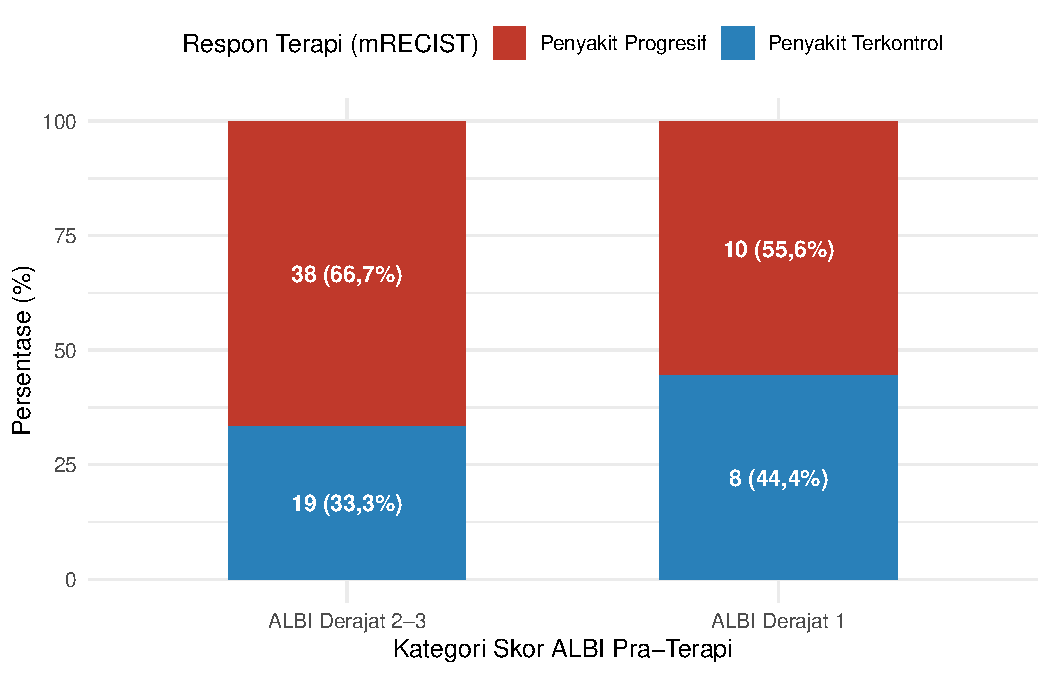
\includegraphics[keepaspectratio]{index_files/figure-pdf/fig-proporsi-albi-1.pdf}}

}

\caption{\label{fig-proporsi-albi}Proporsi penyakit terkontrol
(CR/PR/SD) dan penyakit progresif (PD/ITT) berdasarkan kategori skor
ALBI pra-terapi.}

\end{figure}%

\subsection{Analisis Multivariat (Regresi Logistik Biner) dan Uji
Multikolinearitas}\label{analisis-multivariat-regresi-logistik-biner-dan-uji-multikolinearitas}

Sebanyak 75 subjek dengan data lengkap pada seluruh variabel kandidat
(\(p < 0.25\) pada bivariat dengan missingness \(\le 20\%\)) dimasukkan
ke dalam model regresi logistik biner. Setelah penyesuaian terhadap
variabel perancu, ALBI Derajat 1 menunjukkan adjusted Odds Ratio (aOR)
sebesar 0.86 (95\% CI: 0.13--5.54; \(p =\) 0.873) dengan diskriminasi
model AUC = 0.741 dan nilai VIF maksimum = 2.68
(Tabel~\ref{tbl-multivariat}; Tabel~\ref{tbl-vif};
Gambar~\ref{fig-forest-aor}).

\begin{longtable}[]{@{}
  >{\raggedright\arraybackslash}p{(\linewidth - 8\tabcolsep) * \real{0.3467}}
  >{\raggedright\arraybackslash}p{(\linewidth - 8\tabcolsep) * \real{0.1867}}
  >{\raggedright\arraybackslash}p{(\linewidth - 8\tabcolsep) * \real{0.0800}}
  >{\raggedright\arraybackslash}p{(\linewidth - 8\tabcolsep) * \real{0.2800}}
  >{\raggedright\arraybackslash}p{(\linewidth - 8\tabcolsep) * \real{0.1067}}@{}}

\caption{\label{tbl-multivariat}Hasil Analisis Multivariat Regresi
Logistik Biner Prediktor Penyakit Terkontrol.}

\tabularnewline

\toprule\noalign{}
\begin{minipage}[b]{\linewidth}\raggedright
Variabel Prediktor
\end{minipage} & \begin{minipage}[b]{\linewidth}\raggedright
Koefisien (B)
\end{minipage} & \begin{minipage}[b]{\linewidth}\raggedright
SE
\end{minipage} & \begin{minipage}[b]{\linewidth}\raggedright
Adjusted OR (95\% CI)
\end{minipage} & \begin{minipage}[b]{\linewidth}\raggedright
Nilai p
\end{minipage} \\
\midrule\noalign{}
\endhead
\bottomrule\noalign{}
\endlastfoot
ALBI\_KatALBI Derajat 1 & -0.152 & 0.951 & 0.86 (0.13-- 5.54) & 0.873 \\
Usia\_Kat\textless{} 43 tahun & 1.318 & 0.801 & 3.73 (0.78--17.96) &
0.100 \\
CTP\_KatCTP A & 0.702 & 0.636 & 2.02 (0.58-- 7.01) & 0.270 \\
AFP\_KatAFP \textless200 ng/mL & 0.917 & 0.553 & 2.50 (0.85-- 7.40) &
0.097 \\
PNI\_KatPNI Baik (\textgreater=49.75) & 0.249 & 0.917 & 1.28 (0.21--
7.74) & 0.786 \\
UpToSeven\_KatSesuai (\textless=7) & 1.471 & 0.794 & 4.35 (0.92--20.65)
& 0.064 \\

\end{longtable}

\begin{longtable}[]{@{}lrl@{}}

\caption{\label{tbl-vif}Evaluasi Multikolinearitas Model Multivariat
Berdasarkan Variance Inflation Factor (VIF).}

\tabularnewline

\toprule\noalign{}
Variabel & VIF & Status \\
\midrule\noalign{}
\endhead
\bottomrule\noalign{}
\endlastfoot
ALBI\_Kat & 2.68 & Aman (\textless5) \\
Usia\_Kat & 1.18 & Aman (\textless5) \\
CTP\_Kat & 1.28 & Aman (\textless5) \\
AFP\_Kat & 1.08 & Aman (\textless5) \\
PNI\_Kat & 2.50 & Aman (\textless5) \\
UpToSeven\_Kat & 1.03 & Aman (\textless5) \\

\end{longtable}

\begin{figure}

\centering{

\pandocbounded{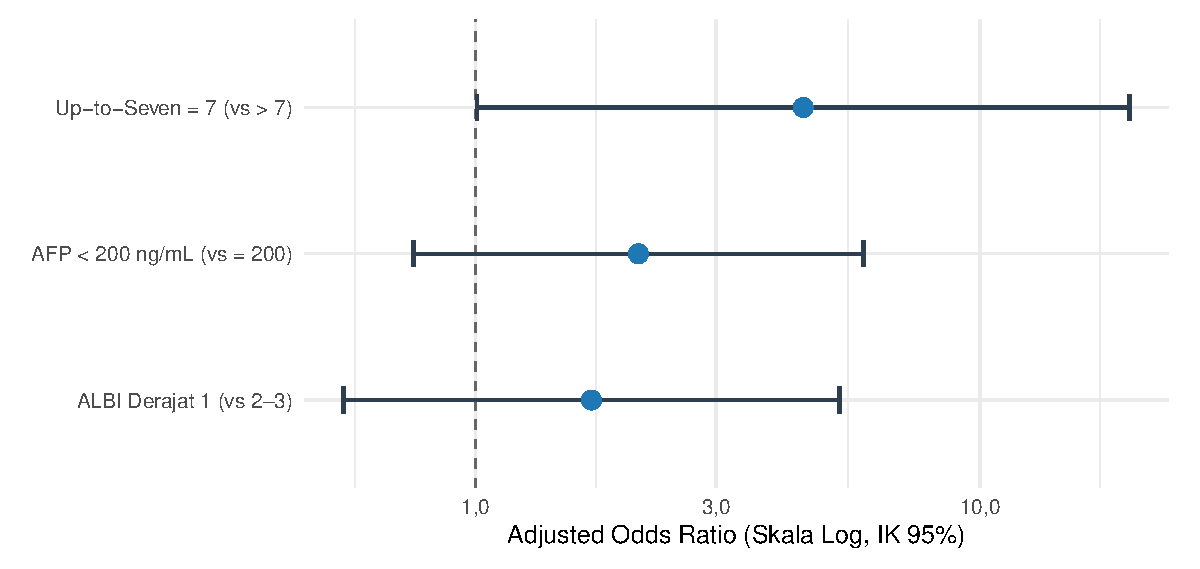
\includegraphics[keepaspectratio]{index_files/figure-pdf/fig-forest-aor-1.pdf}}

}

\caption{\label{fig-forest-aor}Forest plot Adjusted Odds Ratio (aOR) dan
95\% CI dari model regresi logistik biner multivariat.}

\end{figure}%

\section{Pembahasan}\label{pembahasan}

{[}Diisi setelah hasil bivariat dan multivariat terbentuk: bahas
perbandingan dengan studi REFLECT dan kohort Asia Timur, mekanisme
fisiologis ALBI terhadap RDI/tolerabilitas lenvatinib, hasil evaluasi
VIF terhadap CTP/PNI, serta keterbatasan desain retrospektif.{]}

\section{Simpulan}\label{simpulan}

{[}Diisi berdasarkan nilai \(p\) dan aOR akhir skor ALBI
pasca-penyesuaian perancu.{]}

\section{Daftar Pustaka}\label{daftar-pustaka}

\protect\phantomsection\label{refs}
\begin{CSLReferences}{1}{0}
\bibitem[\citeproctext]{ref-johnson2015assessment}
Johnson, P. J., Berhane, S., Kagebayashi, C., Satomura, S., Teng, M.,
Reeves, H. L., O'Beirne, J., Fox, R., Skowronska, A., Palmer, D., Yeo,
W., Mo, F., Lai, P., Iñarrairaegui, M., Chan, S. L., Sangro, B., Miksad,
R., Tada, T., Kumada, T., \& Toyoda, H. (2015). Assessment of {Liver}
{Function} in {Patients} {With} {Hepatocellular} {Carcinoma}: {A} {New}
{Evidence}-{Based} {Approach}---{The} {ALBI} {Grade}. \emph{Journal of
Clinical Oncology}, \emph{33}(6), 550--558.
\url{https://doi.org/10.1200/JCO.2014.57.9151}

\bibitem[\citeproctext]{ref-kudo2018lenvatinib}
Kudo, M., Finn, R. S., Qin, S., Han, K.-H., Ikeda, K., Piscaglia, F.,
Baron, A., Park, J.-W., Han, G., Jassem, J., Blanc, J. F., Vogel, A.,
Komov, D., Evans, T. R. J., Lopez, C., Dutcus, C., Guo, M., Saito, K.,
Kraljevic, S., \ldots{} Cheng, A.-L. (2018). Lenvatinib versus sorafenib
in first-line treatment of patients with unresectable hepatocellular
carcinoma: a randomised phase 3 non-inferiority trial. \emph{Lancet
(London, England)}, \emph{391}(10126), 1163--1173.
\url{https://doi.org/10.1016/S0140-6736(18)30207-1}

\bibitem[\citeproctext]{ref-pphi2017}
Perhimpunan Peneliti Hati Indonesia. (2017). \emph{Konsensus {Nasional}
{Penatalaksanaan} {Karsinoma} {Hati}}. Perhimpunan Peneliti Hati
Indonesia.

\end{CSLReferences}




\end{document}
